\documentclass[11pt,a4paper]{article}
\usepackage[left=2cm, text={17cm,24cm}, top=3cm]{geometry}
\usepackage[czech]{babel}
\usepackage[utf8]{inputenc}
% ROZBÍJÍ TUČNÉ NADPISY
%\usepackage[IL2]{fontenc} %umožňuje vykopírovat správně text s diakritikou
\usepackage{times}
\usepackage[unicode]{hyperref} %pro křížové odkazy
\usepackage{graphicx} %pro práci s obrázky
\usepackage{float}
\usepackage{amsmath} %sazba matematiky
\usepackage[table,xcdraw]{xcolor} %barvičky
\usepackage{listings} %algoritmy, sazba kódu
\usepackage{algpseudocode}
\usepackage{pxfonts}
\usepackage{import}
\usepackage{multicol}
\usepackage{pdflscape}
\usepackage{multicol}
\usepackage{paracol}
\usepackage{enumitem}
\usepackage{longtable}


\newcommand\Alpha{\mathrm{A}} % Alpha
\setlength{\columnsep}{2pt}
\lstset{
  language=C,
  numbersep=5pt,
  breaklines=true,  
  breakatwhitespace=false,
  basicstyle=\ttfamily,
  commentstyle=\color{gray},
  keywordstyle=\bfseries,
  showstringspaces=false,
  %numbers=left,
  %numberstyle=\tiny\color{gray},
}

\begin{document}

\begin{titlepage}
    \begin{center}
        
\includegraphics[height = 160pt]{images/FIT_logo.pdf}\\
		
		{\Huge \textsc{Fakulta informačních technologií}\\[5pt]}
		{\Huge \textsc{Vysoké učení technické v~Brně}}\\
		\vspace{\stretch{0.382}}
		{\LARGE Formální jazyky a překladače\\[5pt]}
		{\LARGE Dokumentace k projektu IFJ a IAL\\[30pt]}
		
		\begin{tabular}{c c c c c}
		    \multicolumn{5}{c}{Tým 128, varianta II}\\[5pt]
            \textbf{Jméno} & \textbf{Příjmení} & \textbf{Xlogin} & \textbf{Rozdělení bodů} & \textbf{Role}\\
            \hline
            Michal & Šmahel & xsmahe01 & 47\% & vedoucí týmu \\[5pt]
            Martin & Havlík & xhavli56 & 45\% &\\[5pt]
            Pavel  & Osinek & xosine00 & 8\% & 
        \end{tabular}\\[30pt]
        \textbf{Implementovaná rozšíření:} žádná
    \end{center}
    \vspace{\stretch{0.609}}
    {
		\hfill
		\today
	}
\end{titlepage}

\newpage
\tableofcontents
\newpage

\section{Úvod}
Cílem projektu bylo vytvořit překladač imperativního programovacího jazyka IFJ21, který vychází z jazyka Teal a překládá se do cílového jazyka IFJcode21. Dokumentace má být velmi stručná (v rozsahu 3-5 stran), takže v ní budou uvedeny zpravidla jen zajímavosti z vývoje a strohý popis jednotlivých částí projektu.
        
\section{Implementace překladače}

Tato sekce se bude věnovat samotné práci na překladači. Způsob organizace práce v týmu a další informace lze nalézt v kapitole \ref{sec:team-work}.

    \subsection{Lexikální analýza}
    V první fázi vývoje jsme se věnovali lexikální analýze a pomocným abstraktním datovým typům, které společně s ní využívají i další funkční celky. Klíčový modul spadající do lexikální analýzy je skener. Ten postupně načítá znaky ze standardního vstupu a pomocí konečného automatu (diagramu je věnována podkapitola \ref{sec:fsm-diagram}) sestavuje tokeny, s nimiž se následně pracuje převážně v syntaktické analýze.
    
    Náš skener na doporučení z přednášky od doktorky Burgetové rovnou ukládá nově nalezené identifikátory do aktuálně nejlokálnější tabulky symbolů. Během syntaktické analýzy je již kostra tabulky připravená a je možné s ní rovnou pracovat. Za poznámku jistě stojí zmínka o tom, jak poznáme, zda byla již proměnná deklarována nebo ji jen skener načetl na pravé straně přiřazení. Tady spoléháme na prostý předpoklad, že deklarovaná proměnná má již u svého identifikátoru uvedeno, že se jedná o proměnnou (nikoliv funkci) a má přidělen typ.
    
    Při tvorbě diagramu jsme využili online simulátoru\cite{fsm-simulator}, který po zadání formální definice automatu generuje ekvivalentní diagram. Tento diagram bylo následně nutné ručně upravit, ale během návrhu konečného automatu nám tento nástroj velmi zpříjemnil práci.
    
        \subsubsection{Diagram konečného automatu}
        \label{sec:fsm-diagram}
        Konečný automat, který je srdcem skeneru, je implementován podle diagramu na obrázku \ref{fig:fsm-diagram}. Pro zvýšení přehlednosti nejsou jednoprvkové množiny přípustných znaků uváděny do složených závorek, stejně tak není uveden chybový stav zajišťující úplnost. Některé rozsáhlejší množiny jsou zastoupeny řeckými písmeny, k nimž se vztahuje následující legenda:
        \begin{itemize}
            \item $\Alpha$ -- znaky A-Z z ASCII tabulky
            \item $\alpha$ -- znaky a-z z ASCII tabulky
            \item $\gamma$ -- znaky 0-9 z ASCII tabulky
            \item $\Sigma$ -- množina všech znaků ASCII tabulky
        \end{itemize}
    
        \begin{figure}[H]
        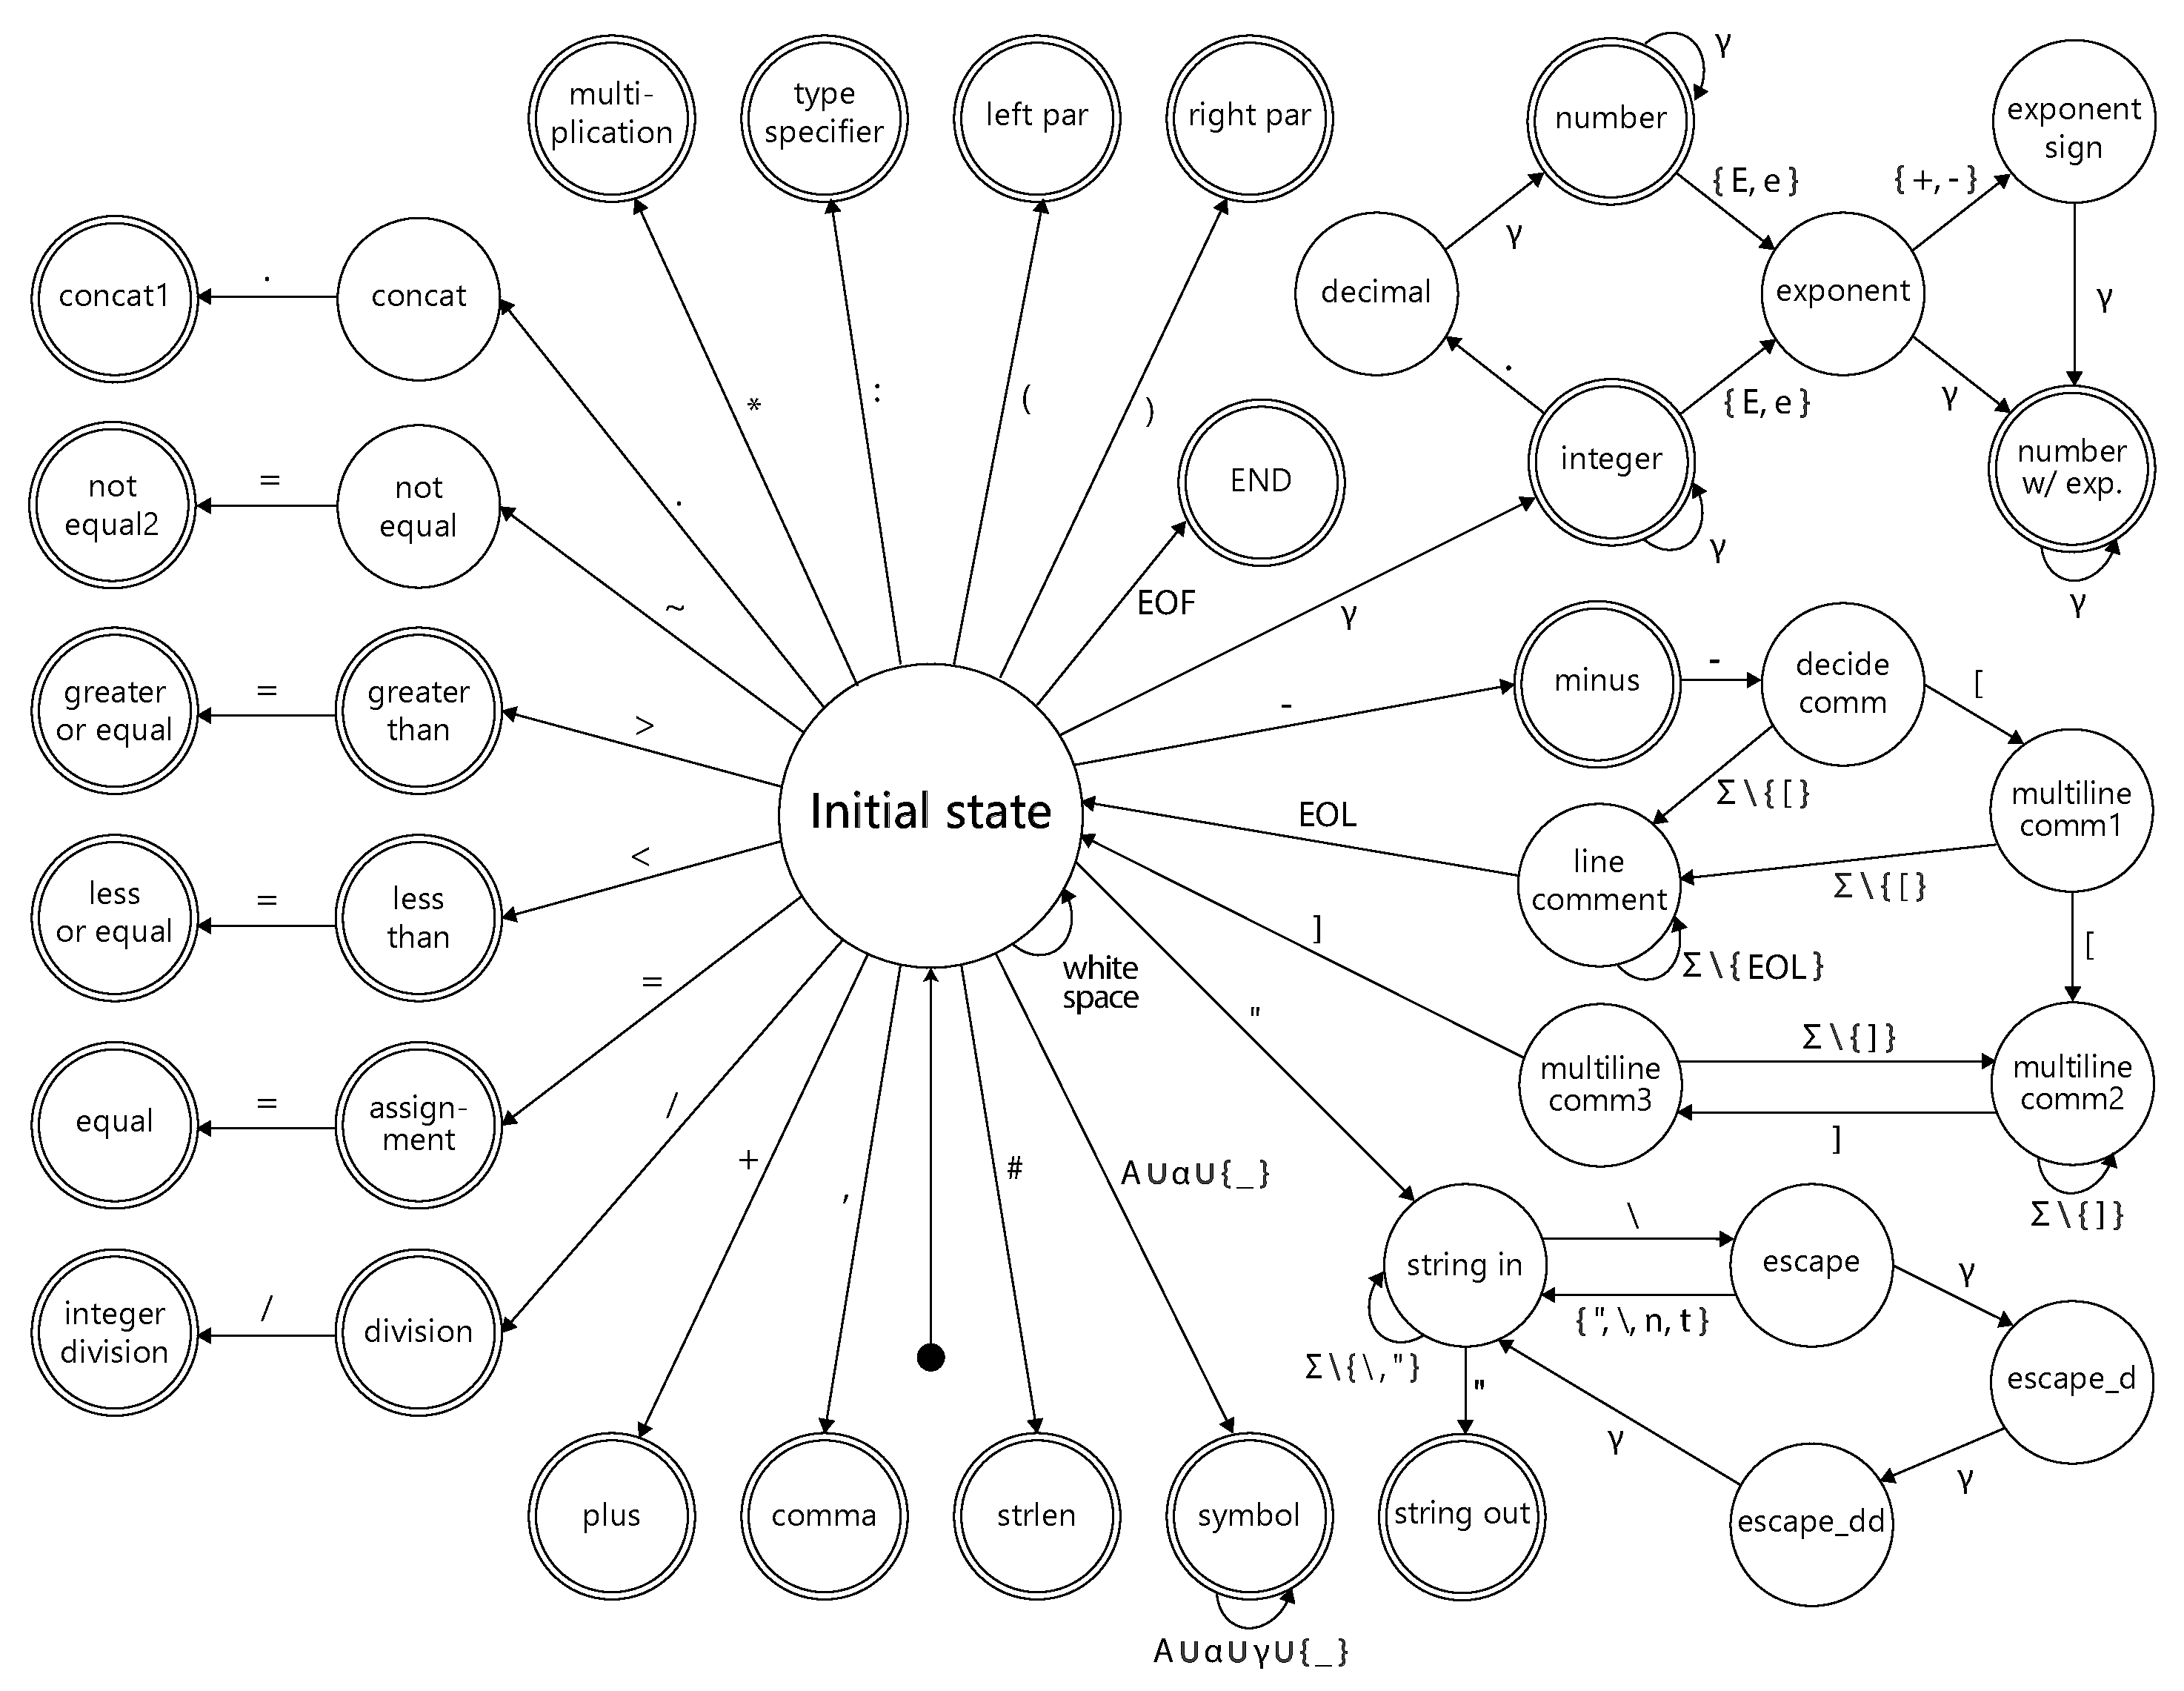
\includegraphics[width=\linewidth]{images/FSM_v12.pdf}
        \caption{Diagram konečného automatu}
        \label{fig:fsm-diagram}
        \end{figure}
    \subsection{Syntaktická analýza}
    Syntaktickou analýzu máme rozdělenou do dvou modulů podle toho, jaká metoda je použita. Metoda shora dolů je implementována v modulu \texttt{parser.c} a zdola nahoru poté v \texttt{expr\_parser.c}. Výhodou tohoto rozdělení bylo, že mohl na každé metodě pracovat jiný člen týmu. Navíc je spolehlivě oddělen kód pro obě z metod, a tedy nedochází k mísení.
    
        \subsubsection{SA shora dolů}
        Při návrhu LL gramatiky (viz níže) jsme využili online nástroj\cite{LL-grammar-simulator} pro  vizualizaci tvorby derivačního stromu a odzkoušení funkčnosti gramatiky. V implementaci jsme potom zvolili doporučenou metodu rekurzivního sestupu, převážně díky její přímočaré realizaci přepisem z pravidel gramatiky. Implementace se nachází v souboru \texttt{parser.c}. Doprovodná LL tabulka se bohužel nevešla na jednu stránku, je tedy dostupná jako tabulka \ref{tab:ll-tab-1} a tabulka \ref{tab:ll-tab-2}.\\
        
        \begin{paracol}{2}
            \noindent
            \verb#1: PROG = REQUIRE CODE#\\
            \verb#2: REQUIRE ::= require "ifj21"#\\
            \verb#3: CODE ::= CODE' CODE''#\\
            \verb#4: CODE ::= ''#\\
            \noindent
            \verb#5: CODE' ::= FUN_DEC#\\
            \verb#6: CODE' ::= FUN_DEF#\\
            \verb#7: CODE' ::= CALL#\\
            \verb#8: CODE'' ::= CODE' CODE''#\\
            \verb#9: CODE'' ::= ''#\\
            \verb#10: FUN_DEC ::= global id : FUN_SIGNATURE#\\
            \verb#11: FUN_SIGNATURE = function (TYPE_LIST) FUN_RET#\\
            \verb#12: TYPE_LIST::= TYPE TYPE_LIST'#\\
            \verb#13: TYPE_LIST::= ''#\\
            \verb#14: TYPE_LIST' ::= , TYPE TYPE_LIST'#\\
            \switchcolumn
            \noindent
            \verb#15: TYPE_LIST' ::= ''#\\
            \verb#16: FUN_RET ::= : FUN_RET_LIST#\\
            \verb#17: FUN_RET ::= ''#\\
            \verb#18: CALL ::= id ( TERM_SEQ )#\\
            \verb#19: TERM_SEQ ::= TERM TERM_SEQ'#\\
            \verb#20: TERM_SEQ ::= ''#\\
            \verb#21: TERM_SEQ' ::= , TERM TERM_SEQ'#\\
            \verb#22: TERM_SEQ' ::= ''#\\
            \verb#23: FUN_RET_LIST ::= TYPE FUN_RET_LIST'#\\
            \verb#24: FUN_RET_LIST' ::= , TYPE FUN_RET_LIST'#\\
            \\
            \verb#25: FUN_RET_LIST' ::= ''#\\
            \verb#26: RET_STMT ::= return RET_E_LIST#\\
            \verb#27: RET_E_LIST ::= E_LIST#\\
            \verb#28: RET_E_LIST ::= ''#\\
            \end{paracol}
            \begin{paracol}{2}
            \noindent
            \verb#29: FUN_DEF = function id (PARAM_LIST) FUN_RET BODY end#\\
            \verb#30: PARAM_LIST ::= PARAM PARAM'#\\
            \verb#31: PARAM_LIST ::= ''#\\
            \verb#32: PARAM ::= id : TYPE#\\
            \verb#33: PARAM' ::= , PARAM PARAM'#\\
            \verb#34: PARAM' ::= ''#\\
            \verb#35: BODY ::= BODY' BODY''#\\
            \verb#36: BODY ::= ''#\\
            \verb#37: BODY' ::= VAR_DEC_DEF#\\
            \verb#38: BODY' ::= STMT#\\
            \verb#39: BODY' ::= IF#\\
            \verb#40: BODY' ::= WHILE#\\
            \verb#41: BODY' ::= RET_STMT#\\
            \verb#42: BODY' ::= CALL#\\
            \verb#43: BODY'' ::= BODY' BODY''#\\
            \verb#44: BODY'' ::= ''#\\
            \verb#45: TERM ::= id#\\
            \verb#46: TERM ::= integer#\\
            \verb#47: TERM ::= number#\\
            \switchcolumn
            \verb##\\
            \verb#48: TERM ::= string#\\
            \verb#49: TERM ::= nil#\\
            \verb#50: VAR_DEC_DEF ::= VAR_DEC VAR_ASSIGN#\\
            \verb#51: VAR_DEC ::= local id : TYPE#\\
            \verb#52: TYPE ::= integer#\\
            \verb#53: TYPE ::= number#\\
            \verb#54: TYPE ::= string#\\
            \verb#55: VAR_ASSIGN ::= = e#\\
            \verb#56: VAR_ASSIGN ::= ''#\\
            \verb#57: STMT ::= ID_SEQ = E_LIST/CALL#\\
            \verb#58: ID_SEQ ::= id ID_SEQ'#\\
            \verb#59: ID_SEQ' ::= , id ID_SEQ'#\\
            \verb#60: ID_SEQ' ::= ''#\\
            \verb#61: E_LIST ::= e E'#\\
            \verb#62: E' ::= , e E'#\\
            \verb#63: E' ::= ''#\\
            \verb#64: IF ::= if e then BODY else BODY end#\\
            \verb#65: WHILE ::= while e do BODY end#
        \end{paracol}

        Porušení LL gramatiky u volání funkcí na pravé straně přiřazení, viz pravidlo gramatiky \verb#57#, a v těle funkce, viz tabulku \ref{tab:ll-tab-1}, řešíme následovně.
        
        Identifikátor reprezentujeme pomocí \texttt{identifier\_t}, který mimo jiné obsahuje informaci, zda se jedná identifikátor proměnné či funkce (viz kapitolu \ref{sec:symtable}). Při zpracování tokenu obsahujícího identifikátor tedy lze rozhodnout, zda zpracovávat levou stranu přiřazení, volat funkci nebo zda přepnout na syntaktickou analýzu zdola nahoru.
        
        %filler
        Přepínání řešíme vcelku jednoduše, dokážeme skeneru vrátit poslední načtený token, který již patří do výrazu. Následně zavoláme funkci, která spustí analýzu metodou zdola nahoru a zpracuje celý výraz až po první nevalidní výrazový token, jenž je opět vrácen skeneru, aby po přepnutí zpět mohl být zpracován SA shora dolů.
        
        \newpage
        \subsubsection{LL-tabulka}
        \begin{table}[ht!]
        \begin{tabular}{|c|c|c|c|c|c|c|c|c|c|c|c|l|}
        \hline
         & \$ & require & global & id & : & function & ( & ) & , & return & end & = \\ \hline
        PROG &  & 1 &  &  &  &  &  &  &  &  &  &  \\ \hline
        REQUIRE &  & 2 &  &  &  &  &  &  &  &  &  &  \\ \hline
        CODE & 4 &  & 3 & 3 &  & 3 &  &  &  &  &  &  \\ \hline
        CODE' &  &  & 5 & 7 &  & 6 &  &  &  &  &  &  \\ \hline
        CODE'' & 9 &  & 8 & 8 &  & 8 &  &  &  &  &  &  \\ \hline
        FUN\_DEC &  &  & 10 &  &  &  &  &  &  &  &  &  \\ \hline
        FUN\_SIGNATURE &  &  &  &  &  & 11 &  &  &  &  &  &  \\ \hline
        TYPE\_LIST &  &  &  &  &  &  &  & 13 &  &  &  &  \\ \hline
        TYPE\_LIST' &  &  &  &  &  &  &  & 15 & 14 &  &  &  \\ \hline
        FUN\_RET & 17 &  & 17 & 17 & 16 & 17 &  &  &  & 17 & 17 &  \\ \hline
        CALL &  &  &  & 18 &  &  &  &  &  &  &  &  \\ \hline
        TERM\_SEQ &  &  &  & 19 &  &  &  & 20 &  &  &  &  \\ \hline
        TERM\_SEQ' &  &  &  &  &  &  &  & 22 & 21 &  &  &  \\ \hline
        FUN\_RET\_LIST &  &  &  &  &  &  &  &  &  &  &  &  \\ \hline
        FUN\_RET\_LIST' & 25 &  & 25 & 25 &  & 25 &  &  & 24 & 25 & 25 &  \\ \hline
        RET\_STMT &  &  &  &  &  &  &  &  &  & 26 &  &  \\ \hline
        RET\_E\_LIST &  &  &  & 28 &  & 29 &  &  &  & 28 & 28 &  \\ \hline
        FUN\_DEF &  &  &  &  &  &  &  &  &  &  &  &  \\ \hline
        PARAM\_LIST &  &  &  & 30 &  &  &  & 31 &  &  &  &  \\ \hline
        PARAM &  &  &  & 32 &  &  &  &  &  &  &  &  \\ \hline
        PARAM' &  &  &  &  &  &  &  & 34 & 33 &  &  &  \\ \hline
        BODY &  &  &  & 35 &  &  &  &  &  & 35 & 36 &  \\ \hline
        BODY' &  &  &  & \cellcolor[HTML]{FFCCC9}38/42 &  &  &  &  &  & 41 & 44 &  \\ \hline
        BODY'' &  &  &  & 43 &  &  &  &  &  & 43 &  &  \\ \hline
        TERM &  &  &  & 45 &  &  &  &  &  &  &  &  \\ \hline
        VAR\_DEC\_DEF &  &  &  &  &  &  &  &  &  &  &  &  \\ \hline
        VAR\_DEC &  &  &  &  &  &  &  &  &  &  &  &  \\ \hline
        TYPE &  &  &  &  &  &  &  &  &  &  &  &  \\ \hline
        VAR\_ASSIGN &  &  &  & 56 &  &  &  &  &  & 56 & 56 & 55 \\ \hline
        STMT &  &  &  & 57 &  &  &  &  &  &  &  &  \\ \hline
        ID\_SEQ &  &  &  & 58 &  &  &  &  &  &  &  &  \\ \hline
        ID\_SEQ' &  &  &  &  &  &  &  &  & 59 &  &  & 60 \\ \hline
        E\_LIST &  &  &  &  &  &  &  &  &  &  &  &  \\ \hline
        E' &  &  &  & 63 &  &  &  &  & 62 & 63 & 63 &  \\ \hline
        IF &  &  &  &  &  &  &  &  &  &  &  &  \\ \hline
        WHILE &  &  &  &  &  &  &  &  &  &  &  &  \\ \hline
        \end{tabular}
        \caption{LL tabulka (1. část)}
        \label{tab:ll-tab-1}
        \end{table}

        \begin{table}
        \begin{tabular}{|c|c|c|c|c|c|l|c|c|c|c|c|}
        \hline
         & integer & number & string & nil & local & výraz & if & then & else & while & do \\ \hline
        PROG &  &  &  &  &  &  &  &  &  &  &  \\ \hline
        REQUIRE &  &  &  &  &  &  &  &  &  &  &  \\ \hline
        CODE &  &  &  &  &  &  &  &  &  &  &  \\ \hline
        CODE' &  &  &  &  &  &  &  &  &  &  &  \\ \hline
        CODE'' &  &  &  &  &  &  &  &  &  &  &  \\ \hline
        FUN\_DEC &  &  &  &  &  &  &  &  &  &  &  \\ \hline
        FUN\_SIGNATURE &  &  &  &  &  &  &  &  &  &  &  \\ \hline
        TYPE\_LIST & 12 & 12 & 12 &  &  &  &  &  &  &  &  \\ \hline
        TYPE\_LIST' &  &  &  &  &  &  &  &  &  &  &  \\ \hline
        FUN\_RET &  &  &  &  & 17 &  & 17 &  &  & 17 &  \\ \hline
        CALL &  &  &  &  &  &  &  &  &  &  &  \\ \hline
        TERM\_SEQ & 19 & 19 & 19 & 19 &  &  &  &  &  &  &  \\ \hline
        TERM\_SEQ' &  &  &  &  &  &  &  &  &  &  &  \\ \hline
        FUN\_RET\_LIST & 23 & 23 & 23 &  &  &  &  &  &  &  &  \\ \hline
        FUN\_RET\_LIST' &  &  &  &  & 25 &  & 25 &  &  & 25 &  \\ \hline
        RET\_STMT &  &  &  &  &  &  &  &  &  &  &  \\ \hline
        RET\_E\_LIST &  &  &  &  & 28 & 27 & 28 &  & 28 & 28 &  \\ \hline
        FUN\_DEF &  &  &  &  &  &  &  &  &  &  &  \\ \hline
        PARAM\_LIST &  &  &  &  &  &  &  &  &  &  &  \\ \hline
        PARAM &  &  &  &  &  &  &  &  &  &  &  \\ \hline
        PARAM' &  &  &  &  &  &  &  &  &  &  &  \\ \hline
        BODY &  &  &  &  & 35 &  & 35 &  & 36 & 35 &  \\ \hline
        BODY' &  &  &  &  & 37 &  & 39 &  &  & 40 &  \\ \hline
        BODY'' &  &  &  &  & 43 &  & 43 &  & 44 & 43 &  \\ \hline
        TERM & 46 & 47 & 48 & 49 &  &  &  &  &  &  &  \\ \hline
        VAR\_DEC\_DEF &  &  &  &  & 50 &  &  &  &  &  &  \\ \hline
        VAR\_DEC &  &  &  &  & 51 &  &  &  &  &  &  \\ \hline
        TYPE & 52 & 53 & 54 &  &  &  &  &  &  &  &  \\ \hline
        VAR\_ASSIGN &  &  &  &  & 56 &  & 56 &  & 56 & 56 &  \\ \hline
        STMT &  &  &  &  &  &  &  &  &  &  &  \\ \hline
        ID\_SEQ &  &  &  &  &  &  &  &  &  &  &  \\ \hline
        ID\_SEQ' &  &  &  &  &  &  &  &  &  &  &  \\ \hline
        E\_LIST &  &  &  &  &  & 61 &  &  &  &  &  \\ \hline
        E' &  &  &  &  & 63 &  & 63 &  & 63 & 63 &  \\ \hline
        IF &  &  &  &  &  &  & 64 &  &  &  &  \\ \hline
        WHILE &  &  &  &  &  &  &  &  &  & 65 &  \\ \hline
        \end{tabular}
        \caption{LL tabulka (2. část)}
        \label{tab:ll-tab-2}
        \end{table}
        \newpage
        
        \subsection{SA zdola nahoru}
        Jádrem naší syntaktické analýzy pro zpracování výrazů je precedenční tabulka (viz tabulku \ref{tab:prec-tab}). Tato tabulka je přesně přepsána do jazyka C s využitím dvojrozměrného statického pole a enumeračních konstant zastupujících znaky \texttt{<}, \texttt{>}, \texttt{=} a prázdnou buňku. Dále máme implementovaný speciální zásobník jako ADT, aby bylo možné zpracovávat tokeny zásobníkovým automatem představeným na přednášce.
        
        Pravidla jsou implementována jako funkce se shodnou signaturou. To nám dovoluje seskupení pravidel do statického pole. Pravidla totiž vyhodnocujeme jejich postupným voláním při procházení zmíněného pole a následným posuzováním navrácené hodnoty. Kromě vyhodnocení, zda dané pravidlo vyhovuje, jsou v těchto funkcích zastoupeny také syntaktické a sémantické kontroly a sémantické akce.
        
        \begin{table}[h!]\centering %better centered, right? Yep :D
            \begin{tabular}{|c|c|c|c|c|c|c|c|c|c|c|c|c|c|c|c|c|c|}
            \hline
             & \# & * & / & // & + & - & .. & \textless{} & \textless{}= & \textgreater{} & \textgreater{}= & == & $\sim$= & ( & ) & term & \$ \\ \hline
            \# &  & \textgreater{} & \textgreater{} & \textgreater{} & \textgreater{} & \textgreater{} & \textgreater{} & \textgreater{} & \textgreater{} & \textgreater{} & \textgreater{} & \textgreater{} & \textgreater{} & \textless{} & \textgreater{} & \textless{} & \textgreater{} \\ \hline
            * & \textless{} & \textgreater{} & \textgreater{} & \textgreater{} & \textgreater{} & \textgreater{} & \textgreater{} & \textgreater{} & \textgreater{} & \textgreater{} & \textgreater{} & \textgreater{} & \textgreater{} & \textless{} & \textgreater{} & \textless{} & \textgreater{} \\ \hline
            / & \textless{} & \textgreater{} & \textgreater{} & \textgreater{} & \textgreater{} & \textgreater{} & \textgreater{} & \textgreater{} & \textgreater{} & \textgreater{} & \textgreater{} & \textgreater{} & \textgreater{} & \textless{} & \textgreater{} & \textless{} & \textgreater{} \\ \hline
            // & \textless{} & \textgreater{} & \textgreater{} & \textgreater{} & \textgreater{} & \textgreater{} & \textgreater{} & \textgreater{} & \textgreater{} & \textgreater{} & \textgreater{} & \textgreater{} & \textgreater{} & \textless{} & \textgreater{} & \textless{} & \textgreater{} \\ \hline
            + & \textless{} & \textless{} & \textless{} & \textless{} & \textgreater{} & \textgreater{} & \textgreater{} & \textgreater{} & \textgreater{} & \textgreater{} & \textgreater{} & \textgreater{} & \textgreater{} & \textless{} & \textgreater{} & \textless{} & \textgreater{} \\ \hline
            - & \textless{} & \textless{} & \textless{} & \textless{} & \textgreater{} & \textgreater{} & \textgreater{} & \textgreater{} & \textgreater{} & \textgreater{} & \textgreater{} & \textgreater{} & \textgreater{} & \textless{} & \textgreater{} & \textless{} & \textgreater{} \\ \hline
            .. & \textless{} & \textless{} & \textless{} & \textless{} & \textless{} & \textless{} & \textless{} & \textgreater{} & \textgreater{} & \textgreater{} & \textgreater{} & \textgreater{} & \textgreater{} & \textless{} & \textgreater{} & \textless{} & \textgreater{} \\ \hline
            \textless{} & \textless{} & \textless{} & \textless{} & \textless{} & \textless{} & \textless{} & \textless{} &  &  &  &  &  &  & \textless{} & \textgreater{} & \textless{} & \textgreater{} \\ \hline
            \textless{}= & \textless{} & \textless{} & \textless{} & \textless{} & \textless{} & \textless{} & \textless{} &  &  &  &  &  &  & \textless{} & \textgreater{} & \textless{} & \textgreater{} \\ \hline
            \textgreater{} & \textless{} & \textless{} & \textless{} & \textless{} & \textless{} & \textless{} & \textless{} &  &  &  &  &  &  & \textless{} & \textgreater{} & \textless{} & \textgreater{} \\ \hline
            \textgreater{}= & \textless{} & \textless{} & \textless{} & \textless{} & \textless{} & \textless{} & \textless{} &  &  &  &  &  &  & \textless{} & \textgreater{} & \textless{} & \textgreater{} \\ \hline
            == & \textless{} & \textless{} & \textless{} & \textless{} & \textless{} & \textless{} & \textless{} &  &  &  &  &  &  & \textless{} & \textgreater{} & \textless{} & \textgreater{} \\ \hline
            $\sim$= & \textless{} & \textless{} & \textless{} & \textless{} & \textless{} & \textless{} & \textless{} &  &  &  &  &  &  & \textless{} & \textgreater{} & \textless{} & \textgreater{} \\ \hline
            ( & \textless{} & \textless{} & \textless{} & \textless{} & \textless{} & \textless{} & \textless{} & \textless{} & \textless{} & \textless{} & \textless{} & \textless{} & \textless{} & \textless{} & = & \textless{} &  \\ \hline
            ) &  & \textgreater{} & \textgreater{} & \textgreater{} & \textgreater{} & \textgreater{} & \textgreater{} & \textgreater{} & \textgreater{} & \textgreater{} & \textgreater{} & \textgreater{} & \textgreater{} &  & \textgreater{} &  & \textgreater{} \\ \hline
            term &  & \textgreater{} & \textgreater{} & \textgreater{} & \textgreater{} & \textgreater{} & \textgreater{} & \textgreater{} & \textgreater{} & \textgreater{} & \textgreater{} & \textgreater{} & \textgreater{} &  & \textgreater{} &  & \textgreater{} \\ \hline
            \$ & \textless{} & \textless{} & \textless{} & \textless{} & \textless{} & \textless{} & \textless{} & \textless{} & \textless{} & \textless{} & \textless{} & \textless{} & \textless{} & \textless{} &  & \textless{} &  \\ \hline
            \end{tabular}
            \caption{Precedenční tabulka}
            \label{tab:prec-tab}
        \end{table}
    
    \subsection{Sémantická analýza}
    Sémantické kontroly a akce jsme vpisovali přímo do jednotlivých funkcí rekurzivního sestupu SA shora dolů a do funkcí představujících aplikovaná pravidla v SA zdola nahoru.
    
    Kromě povinných kontrol máme implementovanou kontrolu dělení nulovým číselným literálem, která se vyhodnocuje již během překladu. Pokud je nula ukryta v proměnné, odhalí se to klasickým způsobem za běhu programu.
    
    \subsection{Generátor cílového kódu}
    Generování kódu řešíme přímo během zpracování tokenů syntaktickými a sémantickými kontrolami. Sémantické akce tak rovnou volají funkce z generátoru, který vypisuje kód na standardní výstup. Rozhodli jsme se pro to poté, co se jeden člen týmu rozhodl snížit svou aktivitu na minimum, kdy jsme si uvědomili, že bychom komplikovanější postup nestihli zhotovit včas.
    
    Bohužel má tento způsob své nevýhody, a museli jsme podniknout několik ústupků. Veškeré funkce (včetně vestavěných) přeskakujeme nepodmíněnými skoky, aby se jejich kód neprováděl, kdy nemá. Nejsou totiž někde na začátku/konci výsledného souboru, ale rozmístěné všude po něm. K vyhodnocování výrazů využíváme převážně zásobníkové instrukce s využitím přirozeného postfixového zpracování syntaktické analýzy zdola nahoru. Deklarace proměnných v cyklech řešíme podobně jako funkce -- kód pro deklaraci všech proměnných objevujících se v cyklech je generován těsně přes koncem funkce, kam se skočí po zavolání funkce. Následně se zpracování vrací na začátek funkce a potřebné proměnné jsou již deklarovány. Na konci provádění funkce se blok s deklaracemi přeskakuje.
    
    \subsection{Tabulka symbolů}
    \label{sec:symtable}
    
    Vybrali jsme si variantu, kde má být tabulka symbolů implementována pomocí tabulky s rozptýlenými položkami, jelikož jsme již měli její základní implementaci z domácího úkolu z předmětu IJC. Jako položku tabulky jsme použili nově vytvořenou strukturu \texttt{identifier\_t} uchovávající potřebné informace o identifikátoru. Mezi ukládané informace patří název, pozice ve vstupním kódu pro jednoznačné pojmenování, typ (proměnná/funkce) a dále specifické informace. Pokud se jedná o proměnnou, zahrnují zejména její typ, v případě funkce pak její signaturu. Kromě toho si uchováváme další informace, které potřebujeme k analýze.
    
    Pro rozsahy platnosti proměnných využíváme \texttt{symstack\_t}, zásobníkový ADT, do kterého si ukládáme ukazatele na nově vzniklé lokální tabulky symbolů pro každý začínající blok. Na konci bloku odpovídající tabulku symbolů (na vrcholu) zase mažeme. Při vyhledávání proměnné začínáme od nejlokálnější tabulky symbolů a postupujeme do globálnějších tabulek, dokud proměnnou nenalezneme nebo neprojdeme všechny tabulky.
    
    \subsection{Implementovaná rozšíření}
    
    Implementace rozšíření nás sice původně lákala, ale nakonec na tuto fázi projektu nezbyl čas, jelikož jsme řešili projekt víceméně ve dvou lidech s občasnými drobnými příspěvky třetího člena. Podrobněji se této problematice věnuje kapitola \ref{sec:tasks-division}.
    
\section{Práce v týmu}
\label{sec:team-work}

V této kapitole bych z pozice vedoucího týmu rád popsal, jakým způsobem fungoval náš tým, uvedl pár informací k organizaci práce v týmu, dělení úkolů a přidělování bodových částí.

\subsection{Způsob práce na projektu}
\label{sec:way-to-work-on-project}

Na projektu měli pracovat všichni členové týmu. Projekt byl rozdělen na větší množství menších podproblémů s různou mírou složitosti. Rozdělení do úkolů, jejich správu a dohled nad jejich řešením měl na starost vedoucí týmu. O tom, jaký úkol bude kdo vypracovávat však nebylo explicitně rozhodováno, každý člen si mohl zvolit, na čem bude v danou chvíli pracovat. Byla snaha rozdělit úkoly do minimalistických celků, aby se každý člen týmu mohl podílet na řešení každé části vývoje kompilátoru, pokud by měl zájem. Jako příklad lze uvést fakt, že byl každý pomocný abstraktní datový typ vyčleněn do samostatného úkolu.

Cílem bylo, aby měl každý člen alespoň základní povědomí o všech částech projektu. Kvůli tomu, že na jednom větším celku (např. lexikální analýza) pracovalo větší množství lidí, byla také podněcována jejich vzájemná komunikace, při níž bylo třeba domlouvat rozhraní mezi jednotlivými moduly. Nebyl tedy zvolen postup, kdy se rozdělí větší celky a poté se provádí jejich kompozice.

\subsection{Využité nástroje a procesy}

Kvůli jednoduší spolupráci na tvorbě projektu jsme se rozhodli využít verzovací systém Git se vzdáleným repozitářem hostovaným službou Github. Na této službě jsme kromě funkce vzdáleného repozitáře pro správu verzí projektu využili také několik dalších funkcí:
\begin{itemize}
    \item Github project boards\cite{gh-proj-boards} pro organizaci úkolů a jasný přehled o aktuálním stavu projektu,
    \item Github issues\cite{gh-issues} a jako reprezentaci úkolů,
    \item Github pull requests\cite{gh-pull-requests} pro jednoduší, přehlednější a interaktivnější revize kódu,
    \item Github Actions\cite{gh-actions} pro automatizaci úkolů, spouštění automatických testů a kontrol,
    \item Github API\cite{gh-api} pro účely skriptu pro výpočet bodového rozdělení.
\end{itemize}

Služba Github dále poskytuje různé možnosti omezení přístupu k větvím a určitým typům změn\cite{gh-protected-branches}. Díky tomu bylo možné uzamknout výchozí větev a pro veškeré změny vynucovat revize od jiného člena týmu. Autor změn tak vždy dostal zpětnou vazbu od někoho dalšího a podařilo se tak odhalit mnoho chyb, kterých si autor nevšiml. Začleňování změn do hlavní větve bylo prováděno výhradně pomocí webového rozhraní pro žádosti o začlenění změn (běžněji známo pod anglickým pojmem \uv{pull request}). Tam je možné změny komentovat a navrhovat různé úpravy a opravy chyb nalezených během revize.

Samotné psaní kódu si pak členové týmu zařídili po svém podle toho, co komu vyhovovalo. K dispozici byla poměrně komplexní konfigurace nástroje Make\cite{make-official-docs}\cite{make-cheatsheet}, která poskytovala automatickou kompilaci a sestavování zdrojových kódů, jednotkových a manuálních testů, přípravu výsledného archivu pro odevzdání a další drobnosti. Pro jednotkové (\uv{unit}) testy využíváme minimalistický framework Unity\cite{unity}.

\subsection{Rozdělení úkolů}
\label{sec:tasks-division}

Jak bylo zmíněno v kapitole \ref{sec:way-to-work-on-project}, členové týmu si mohli sami volit, čemu se budou věnovat. Jelikož se některé větší úkoly dále špatně dělí, každý člen se nakonec některým částem vývoje kompilátoru věnoval více než jiným, a s trochou nadsázky by se dalo říct, že se na ně \uv{specializoval}. V následujících odstavcích bude rozvedeno rozdělení klíčových částí mezi členy projektu.

Lexikální analýze se primárně věnoval Michal Šmahel. Tato část byla však značně rozdělena i mezi další členy týmu, kteří spolupracovali na pomocných implementacích. Diagram lexikální analýzy (viz obrázek č. \ref{fig:fsm-diagram}) skládali všichni členové týmu na prezenční schůzce. Dále se vytvářely různé pomocné datové struktury, kterým se mimo Michala Šmahela věnoval i Martin Havlík a částečně také Pavel Osinek.

Syntaktická a sémantická analýza byla rozdělena mezi Michala Šmahela a Martina Havlíka. Zpracování struktury zdrojových souborů pomocí metody shora dolů se ujal Martin Havlík, zpracování výrazů metodou zdola nahoru se poté zabýval Michal Šmahel. Ten však řešil pouze implementaci, precedenční tabulku skládal Martin Havlík. Sémantické kontroly a akce následně doplňoval každý do svého modulu sám.

Generování kódu se věnoval opět Michal Šmahel s Martinem Havlíkem. Základní principy generování vymýšleli na týmových schůzkách, kam většinou Pavel Osinek z různých důvodů nedocházel. Implementaci hlavní části následně provedl Martin Havlík s drobnými zásahy (převážně optimalizace generovaného kódu) od Michala Šmahela. Ten kromě toho kompletně vypracoval generování kódu pro vestavěné funkce.

Michal Šmahel se dále, coby vedoucí týmu, podílel na organizaci práce a dohledu na ostatní členy týmu. Rovněž se významně podílel a přípravě pracovního prostředí a testů. Pavel Osinek připravoval šablonu dokumentace a grafickou podobu diagramu stavového automatu.

Důvodem, proč tato kapitola nabývá nadměrné délky, je problém s jedním členem týmu, který se rozhodl projektu věnovat minimum času a úsilí, což bylo nutné dále řešit nerovnoměrným rozdělením bodů. Kvůli této záležitosti byl osloven i dr. Křivka, který povolil výrazné snížení bodů Pavlu Osinkovi, pokud bude dostatečně prokazatelné, kdo měl na čem jaký podíl. Dohodli jsme se na zavedení bodového systému k úkolům zmíněným v kapitole \ref{sec:way-to-work-on-project}, podle něhož se následně spočítala procenta a po drobné korekci v řádu malých jednotek procent prohlásila za finální rozdělení bodů. Doufám, že tato kapitola splnila svůj účel a dokreslila, jakým způsobem se jednotliví členové na projektu podíleli a výsledné bodové rozdělení je tím dostatečně odůvodněné. V případě problémů jsou je k dispozici historie úkolů a jejich bodování včetně automatického hodnotícího skriptu.

\section{Závěr}
Ačkoliv jsme se poslední dva týdny před odevzdáním projektu báli, abychom ve dvou vše stihli dokončit, nakonec se nám to podle našeho názoru podařilo poměrně uspokojivě. Víme sice o několika nedokonalostech, které projekt tíží, ale celkově jsme se svými výkony poměrně spokojení.

Projekt byl velmi zajímavý a jsme rádi, že jsme si mohli zkusit něco takového navrhnout a naprogramovat. Díky negativní zkušenosti máme také jisté ponaučení ohledně práce v týmu, což se nám jistě bude v životě hodit.

\newpage

\section{Zdroje}
    \bibliographystyle{czechiso}
    \bibliography{references}

%     Zkouška citace~\cite{MedunaAlexander2008Eocd}.
    
%     Ukázka \uv{českých} uvozovek.
    
%     Ukázka kódu
%     \begin{lstlisting}
% #include <stdio.h>

% int main() {
%     // printf() displays the string inside quotation
%     printf("Hello, World!");
%     return 0;
% }\end{lstlisting}
          
%     \begin{algorithmic}
%         \State $i \gets 10$
%         \If{$i\geq 5$} 
%             \State $i \gets i-1$
%         \Else
%             \If{$i\leq 3$}
%                 \State $i \gets i+2$
%             \EndIf
%         \EndIf 
%     \end{algorithmic}        

\end{document}
